\begin{figure}
  \centering
  \begin{subfigure}[b]{\textwidth}
    \centering
    
\includegraphics[width=0.6\textwidth]{img/bioscheme}
    \caption{biological inspiration}
    \label{subfig:bioscheme}
  \end{subfigure}
  \hfill
  \begin{subfigure}[b]{0.6\textwidth}
    \centering
    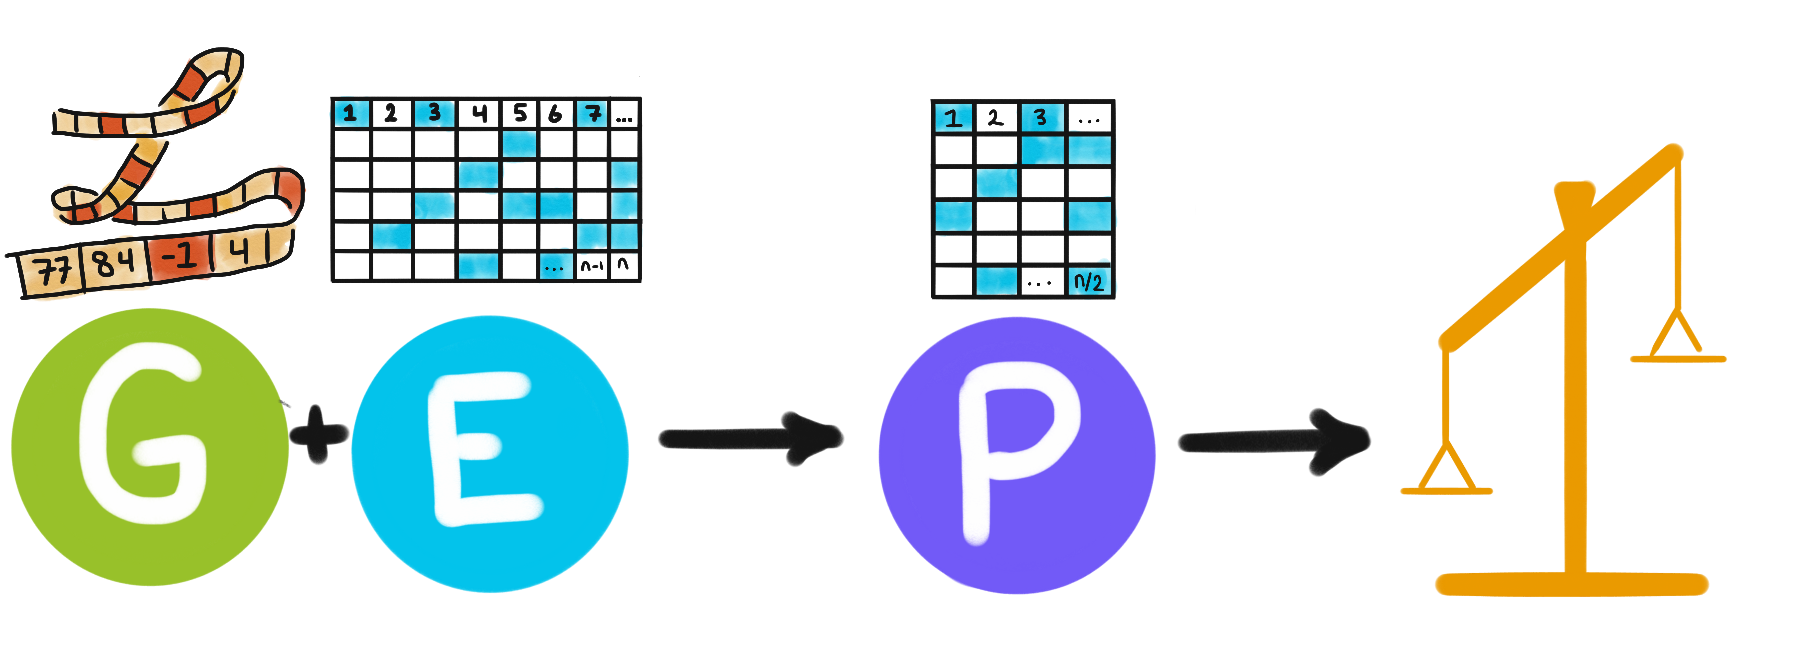
\includegraphics[width=\textwidth]{img/modelscheme}
    \caption{genetic regulatory network model}
     \label{subfig:modelscheme}
  \end{subfigure}
  \captionsetup{singlelinecheck=off,justification=raggedright}
  \caption{A comparison of the genetic regulatory network model and its biological inspiration.}
  \label{fig:model_bio_comparison}
\end{figure}